\chapter{Majoron Decay Search}

\section{Background Sources in CUORE}
What all contributes to the background? Descrive connections to the previous values and from data from CUORE-0. Namely, should have tower sources as the same, and contributions from Cryostat new.
\section{JAGS Analysis Software}
\subsection{Markov Chain Monte Carlo}
\label{ssec:MCMC}

describe how MCMC works exactly. Why does it give proper results? How should it be done properly
To perform a search for a spectrum-based rare event, it 
\section{Source Reconstruction}
How do we put sources into the background fit?
\section{Majoron Analysis}
When fitting the data with JAGS, the spectrum is split into two main components: the \Mone~spectrum, the \Mtwo~spectrum, and the summed \Msum~spectrum. This is done as the signal events from a Majoron search mostly deposit energy into a single crystal, as is typical of events originating from the bulk of the crystal volume, whereas many other sources that are external to a crystal or on the surface have a much higher probability of depositing energy into more than one crystal. Higher multiplicity spectra are not used, except for identifying the contribution of muons to the background, as they do not add significant information to the fit for other sources. For the fit, each of the possible Majoron spectral indices are considered independently and are shown for each multiplicity in \autoref{fig:SpectralIndicesM1Fit} and \autoref{fig:SpectralIndicesM2Fit}.


\begin{figure}[htbp]
\centering
\begin{subfigure}[t]{0.49\textwidth}
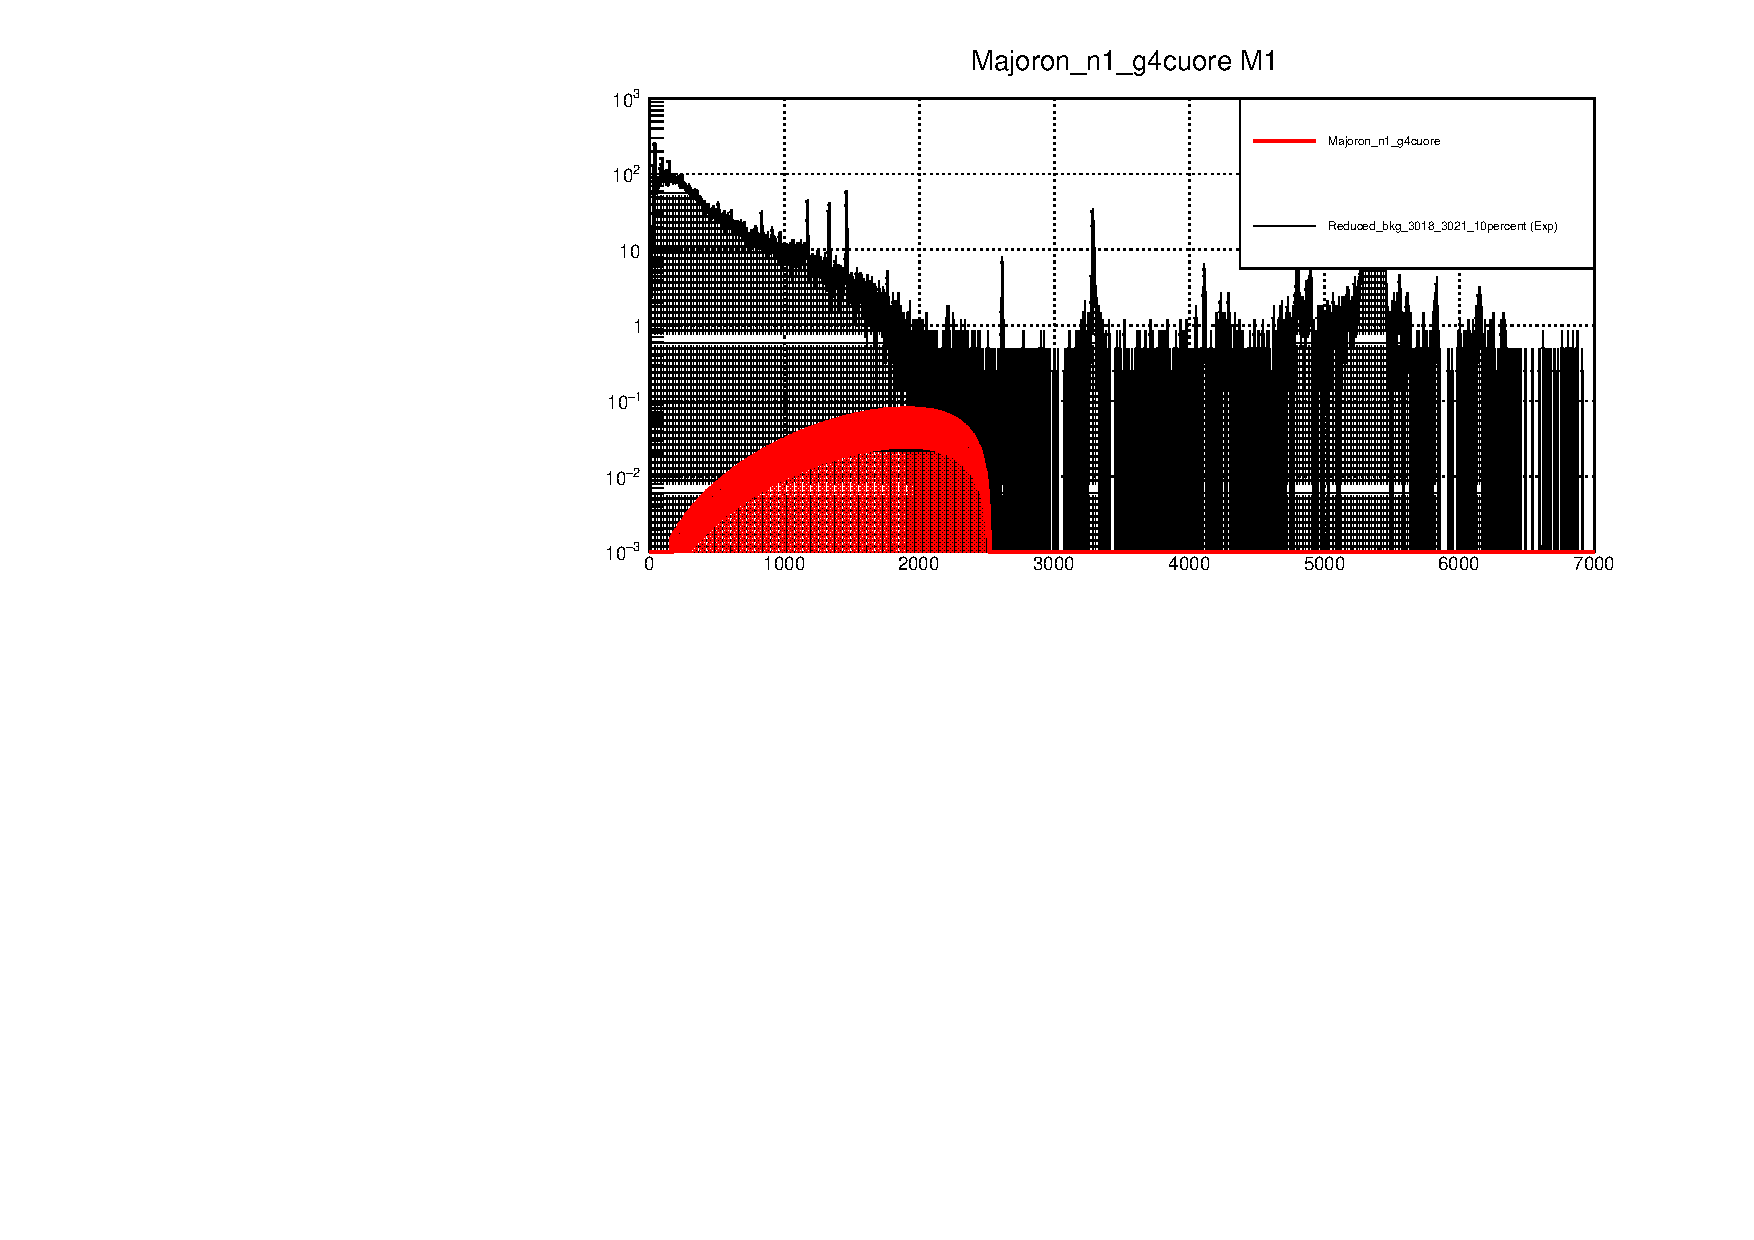
\includegraphics[width=0.9\textwidth]{Figures/Majoron_n1_g4cuore.pdf}
\end{subfigure}
\qquad
\begin{subfigure}[t]{0.49\textwidth}
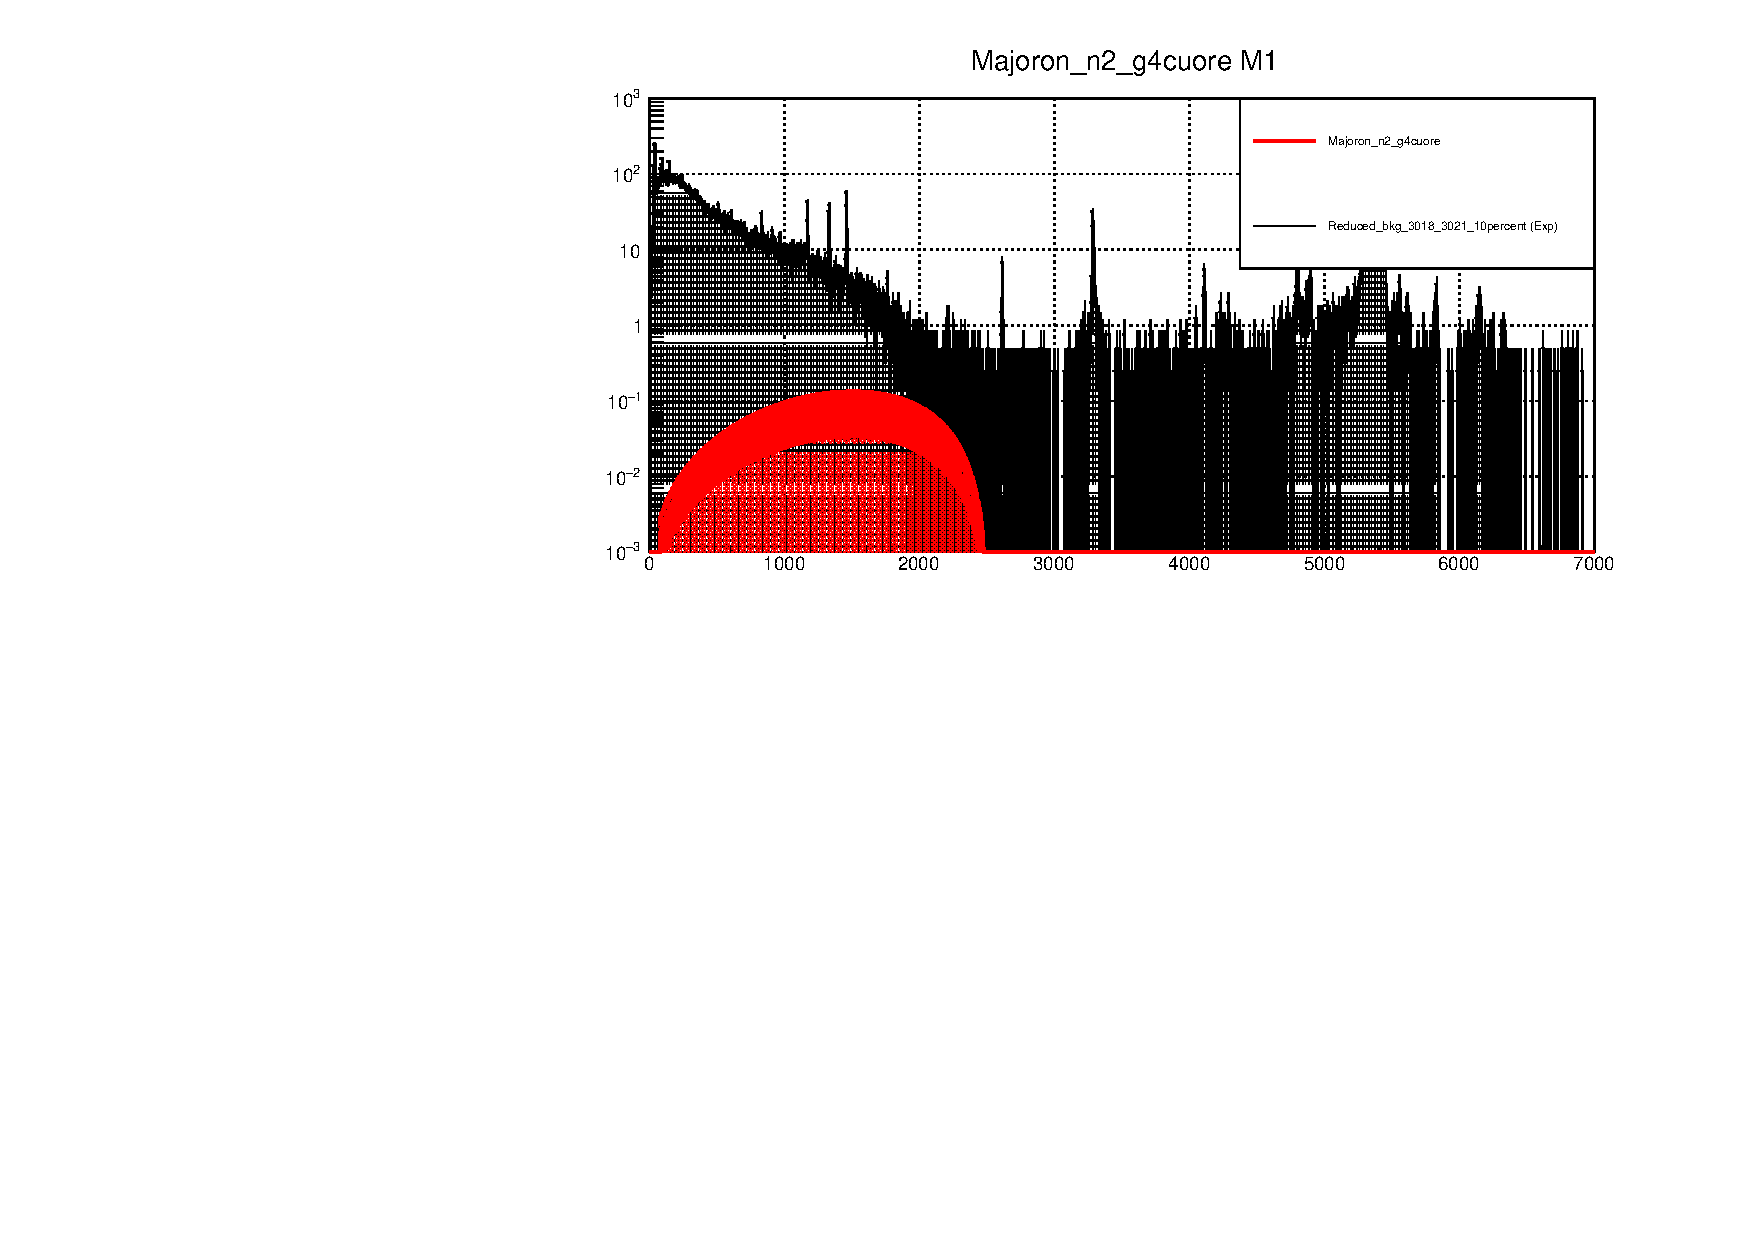
\includegraphics[width=0.9\textwidth]{Figures/Majoron_n2_g4cuore.pdf}
\end{subfigure}
\qquad
\begin{subfigure}[t]{0.49\linewidth}
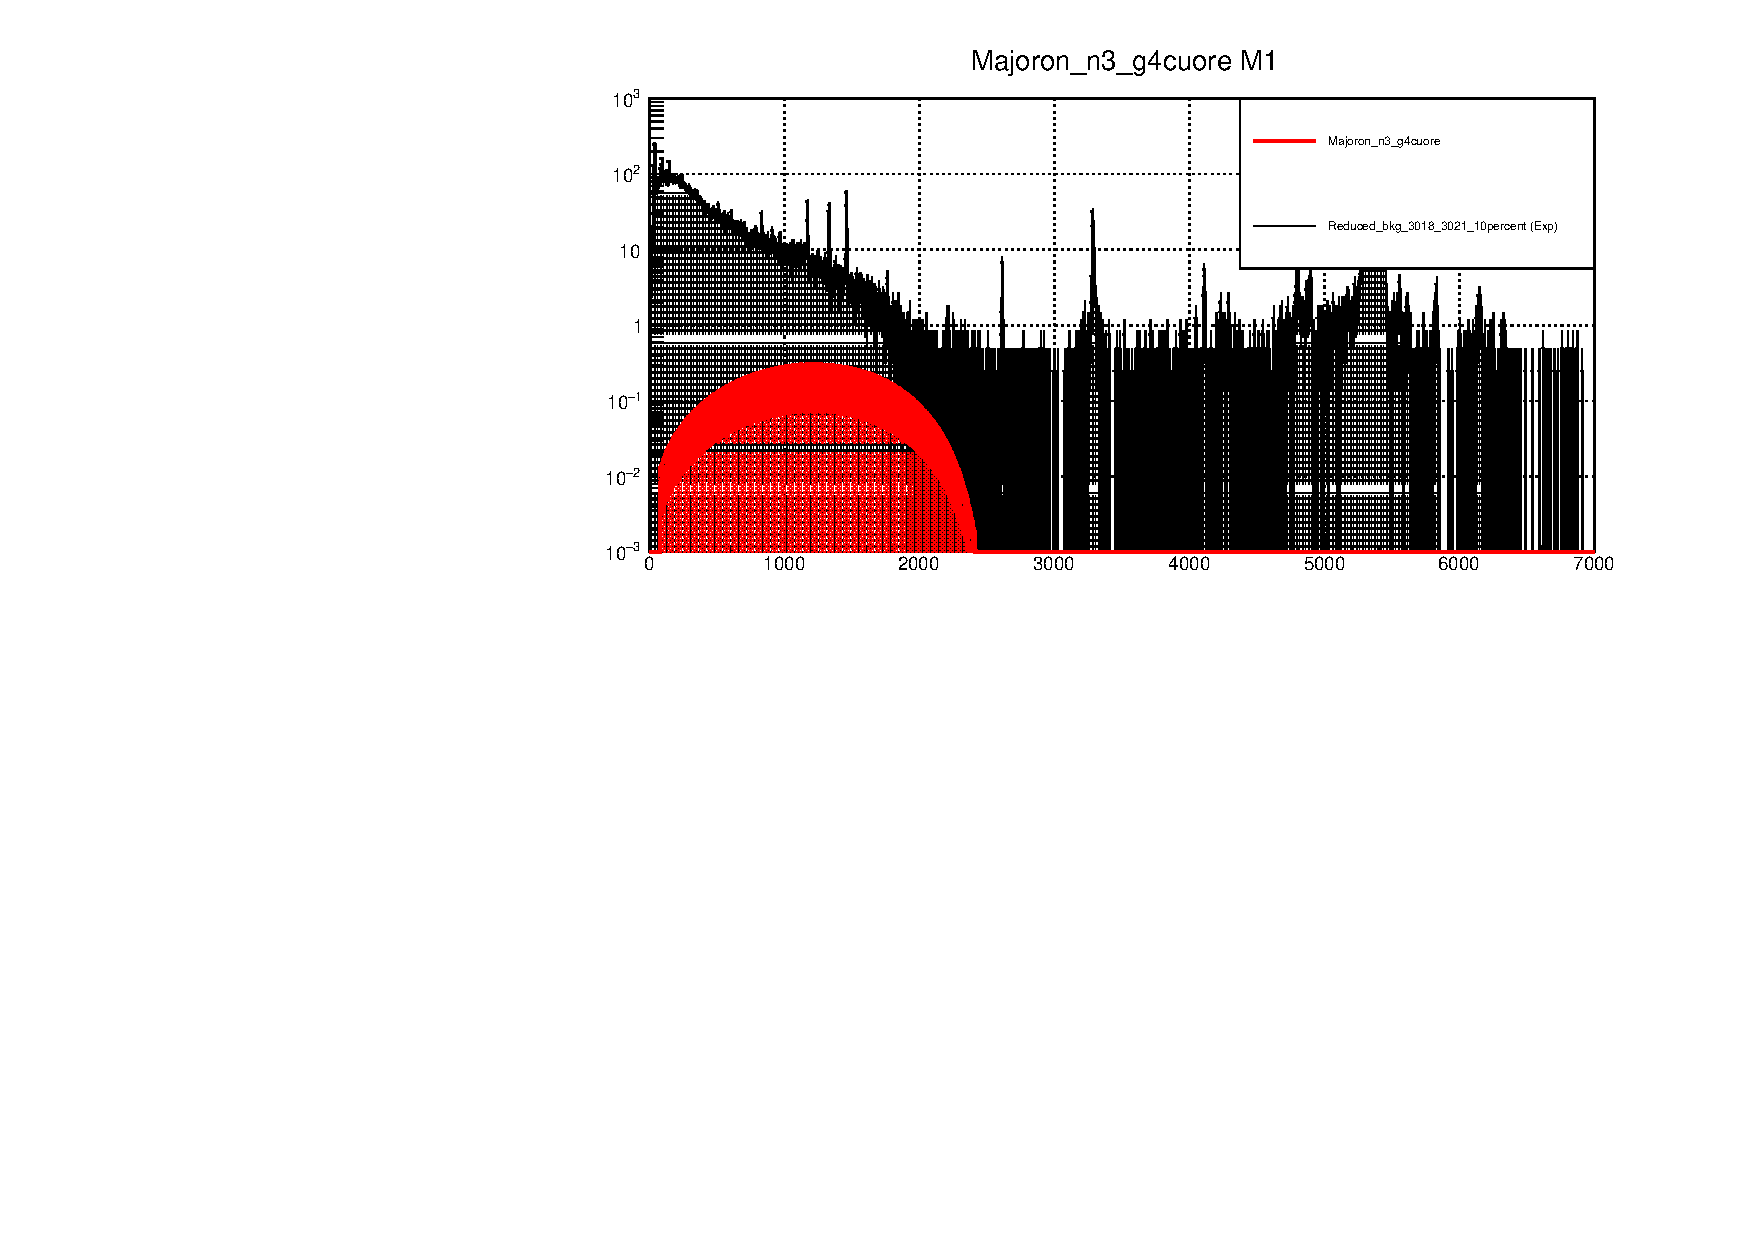
\includegraphics[width=0.9\textwidth]{Figures/Majoron_n3_g4cuore.pdf}
\end{subfigure}
\qquad
\begin{subfigure}[t]{0.49\linewidth}
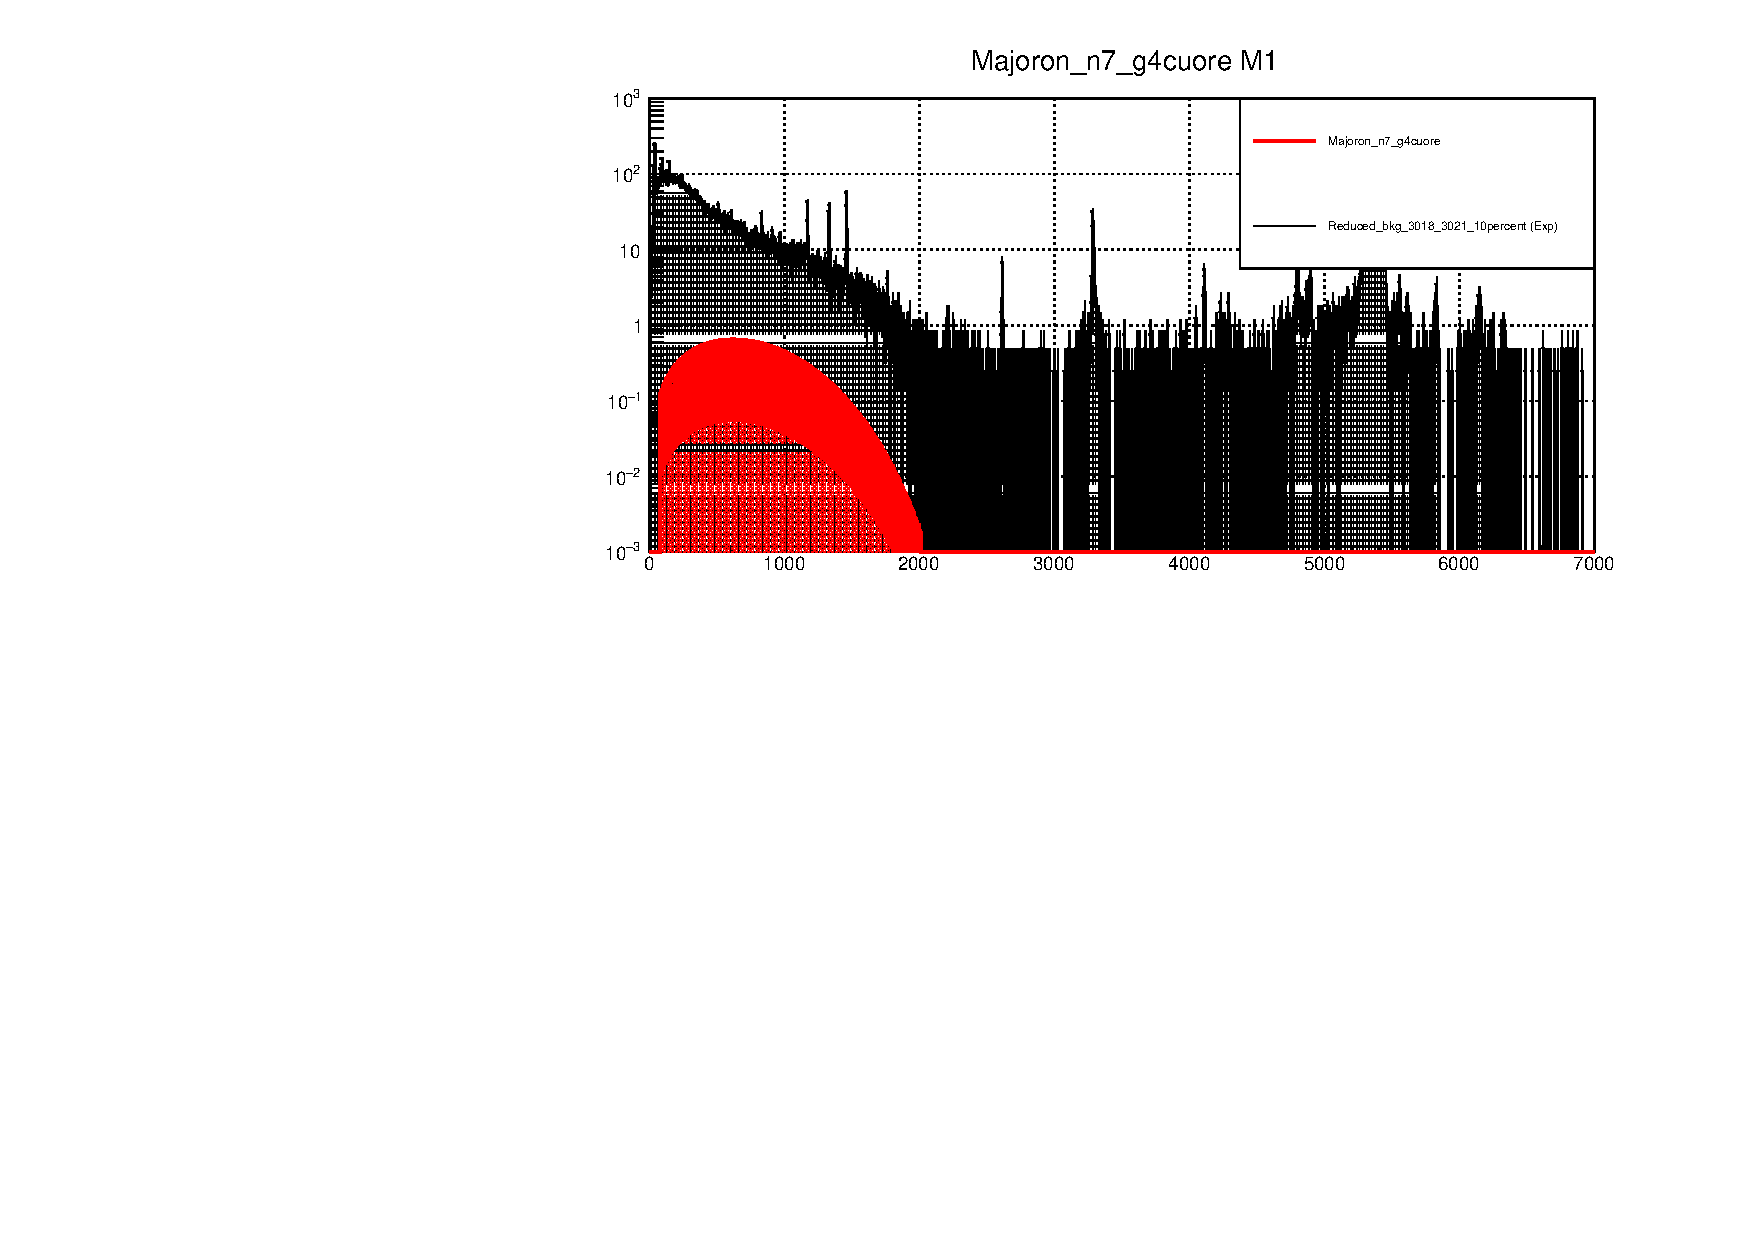
\includegraphics[width=0.9\textwidth]{Figures/Majoron_n7_g4cuore.pdf}
\end{subfigure}
\caption[The fitted contribution of Majoron decays for the different spectral indices in the \Mone~ spectrum.]{The fitted contribution of Majoron decays for the different spectral indices in the \Mone~ spectrum.}
\label{fig:SpectralIndicesM1Fit}
\end{figure}

\begin{figure}[htbp]
\centering
\begin{subfigure}[t]{0.49\textwidth}
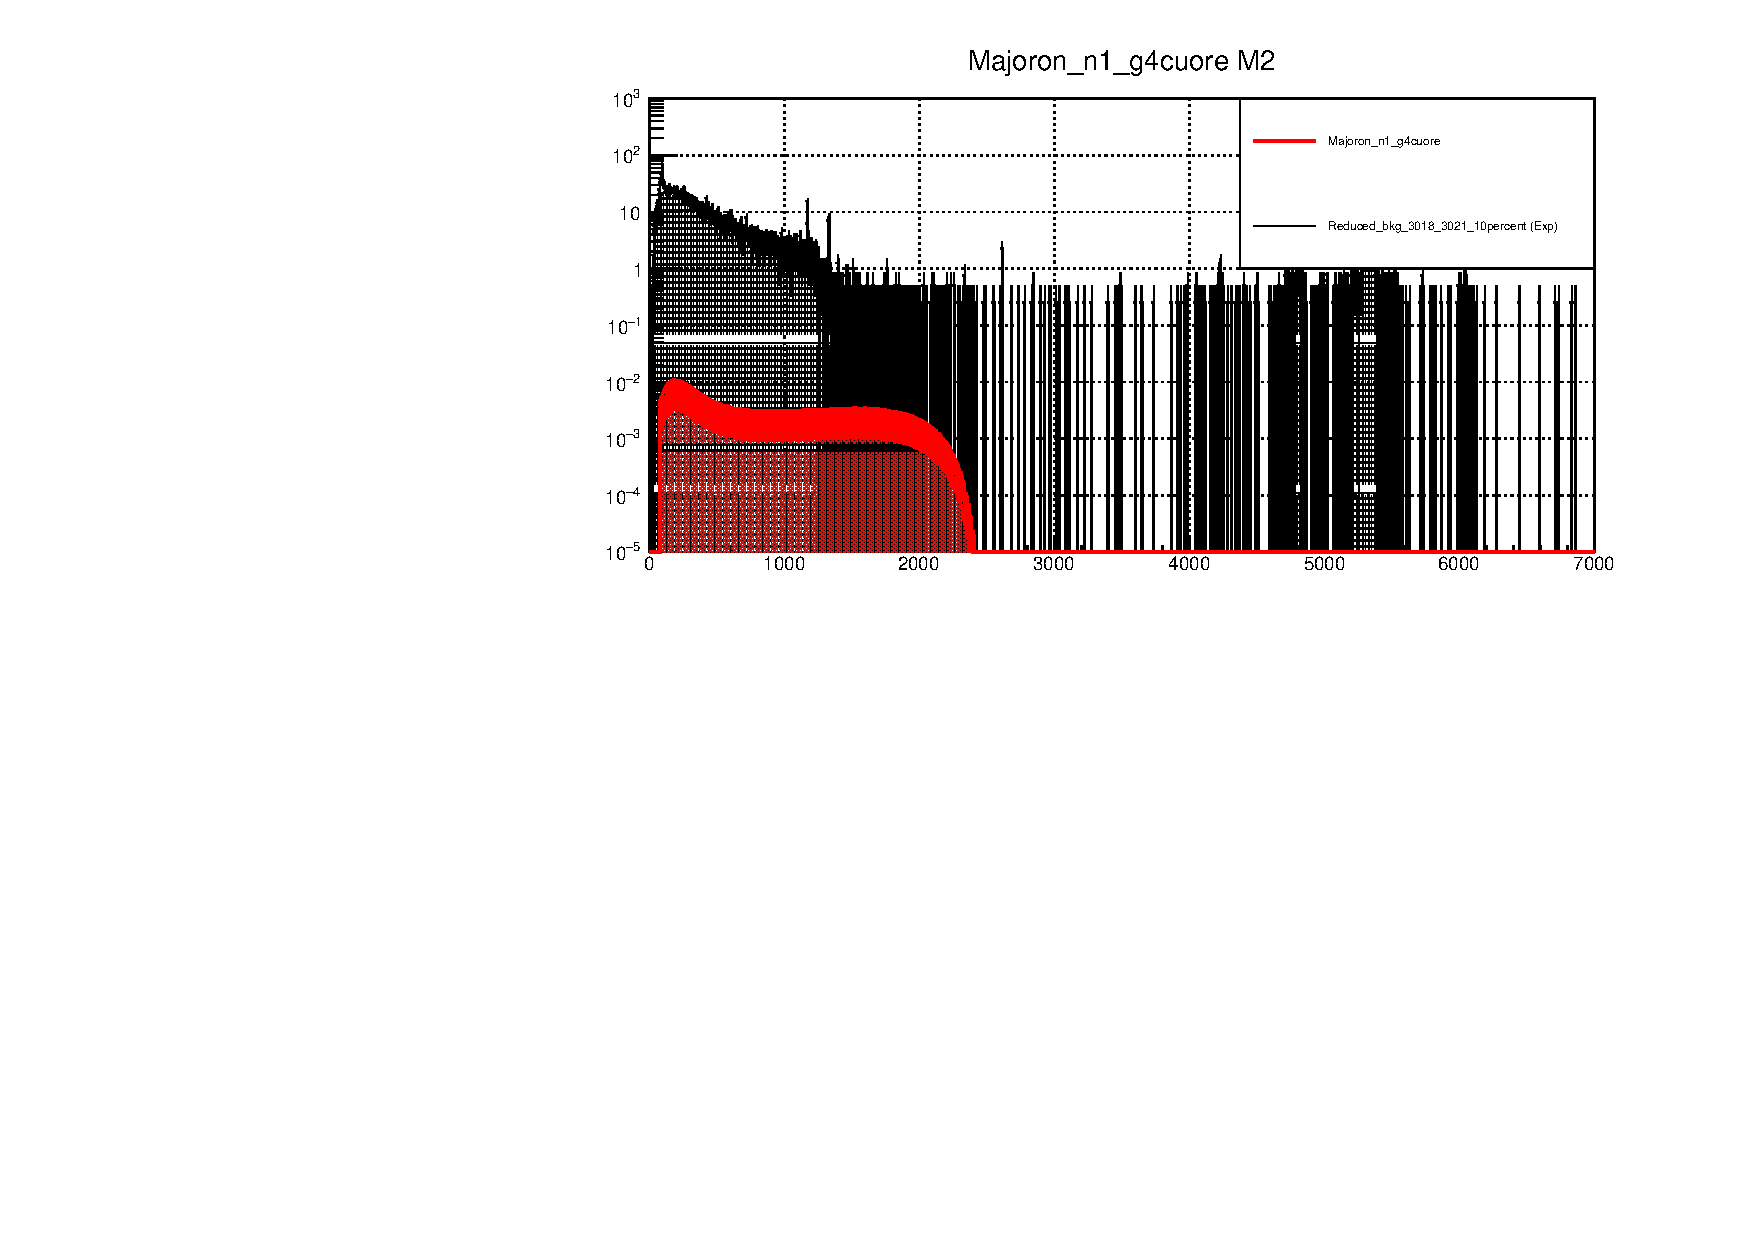
\includegraphics[width=0.9\textwidth]{Figures/Majoron_n1_g4cuore_M2.pdf}
\end{subfigure}
\qquad
\begin{subfigure}[t]{0.49\textwidth}
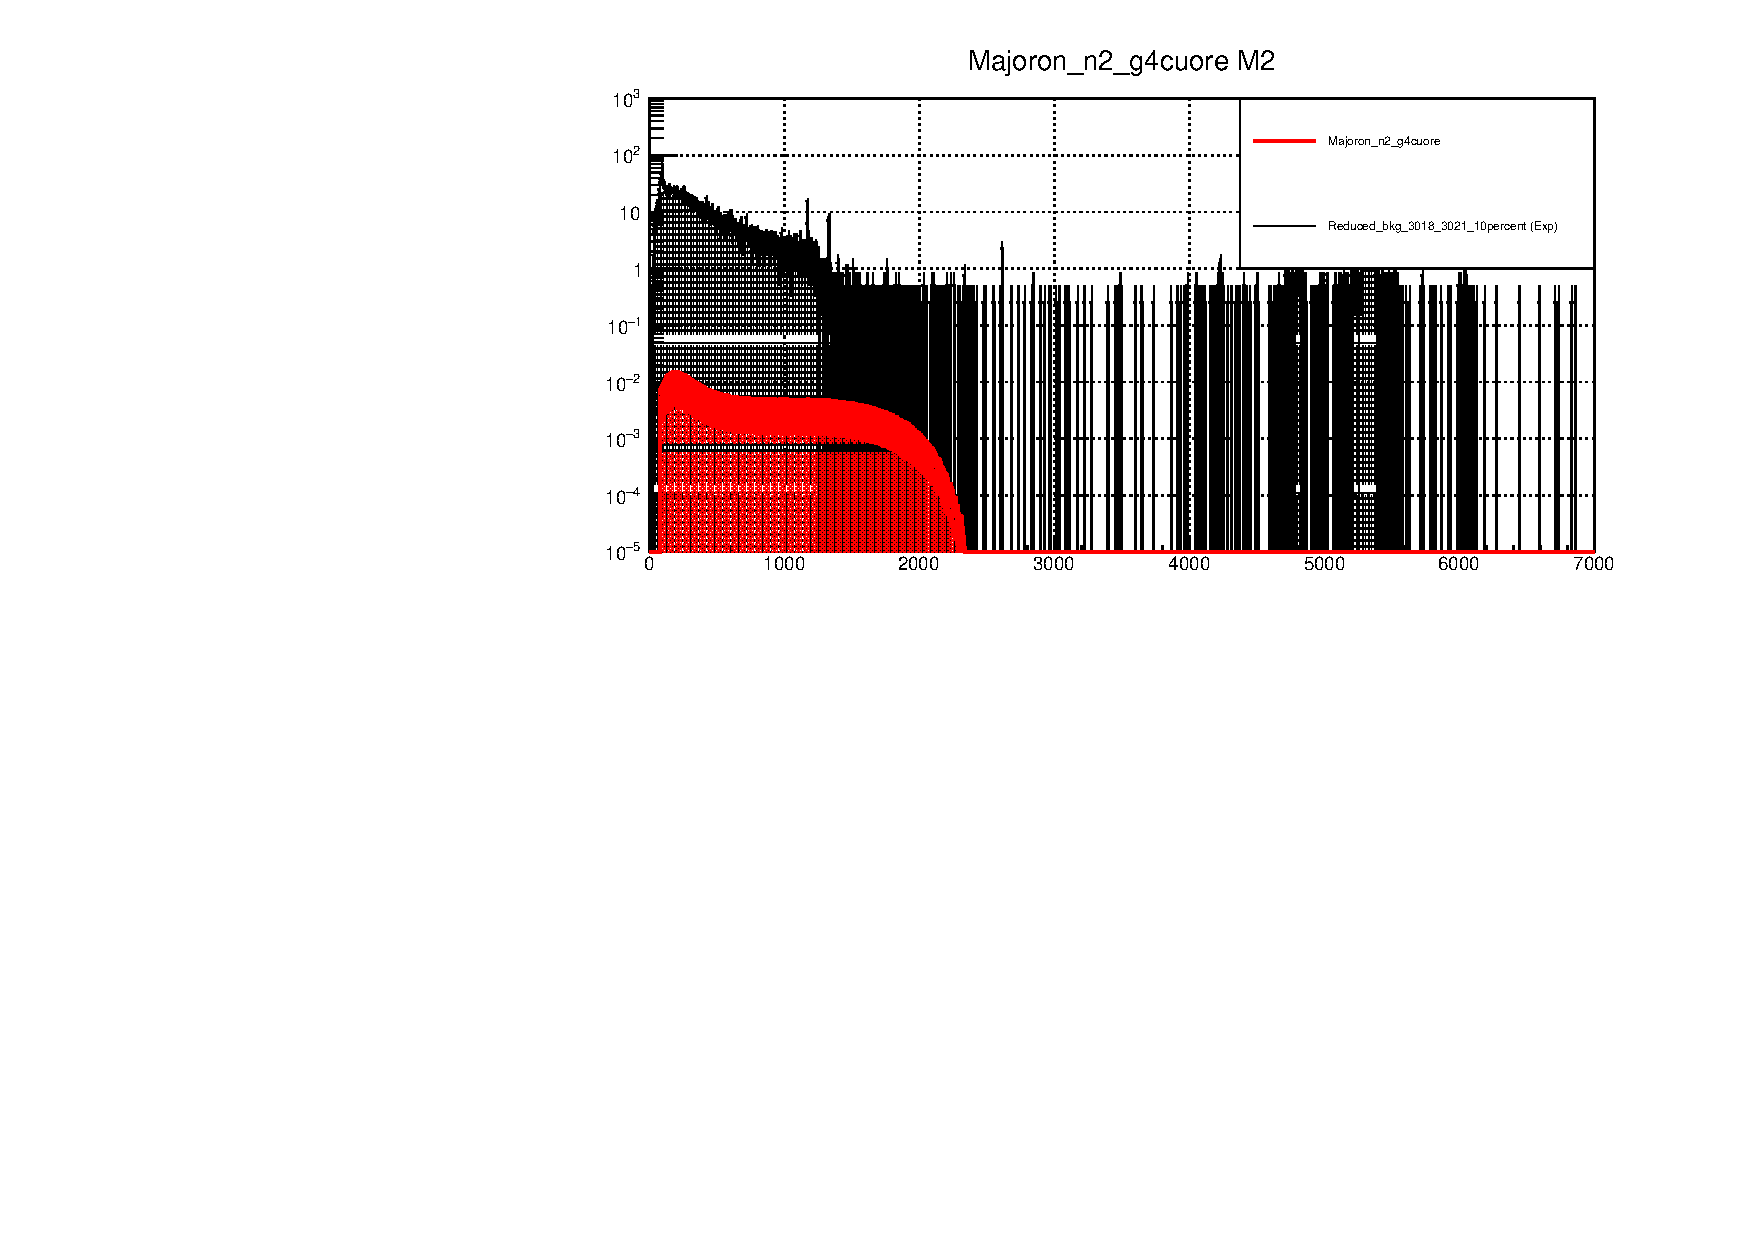
\includegraphics[width=0.9\textwidth]{Figures/Majoron_n2_g4cuore_M2.pdf}
\end{subfigure}
\qquad
\begin{subfigure}[t]{0.49\linewidth}
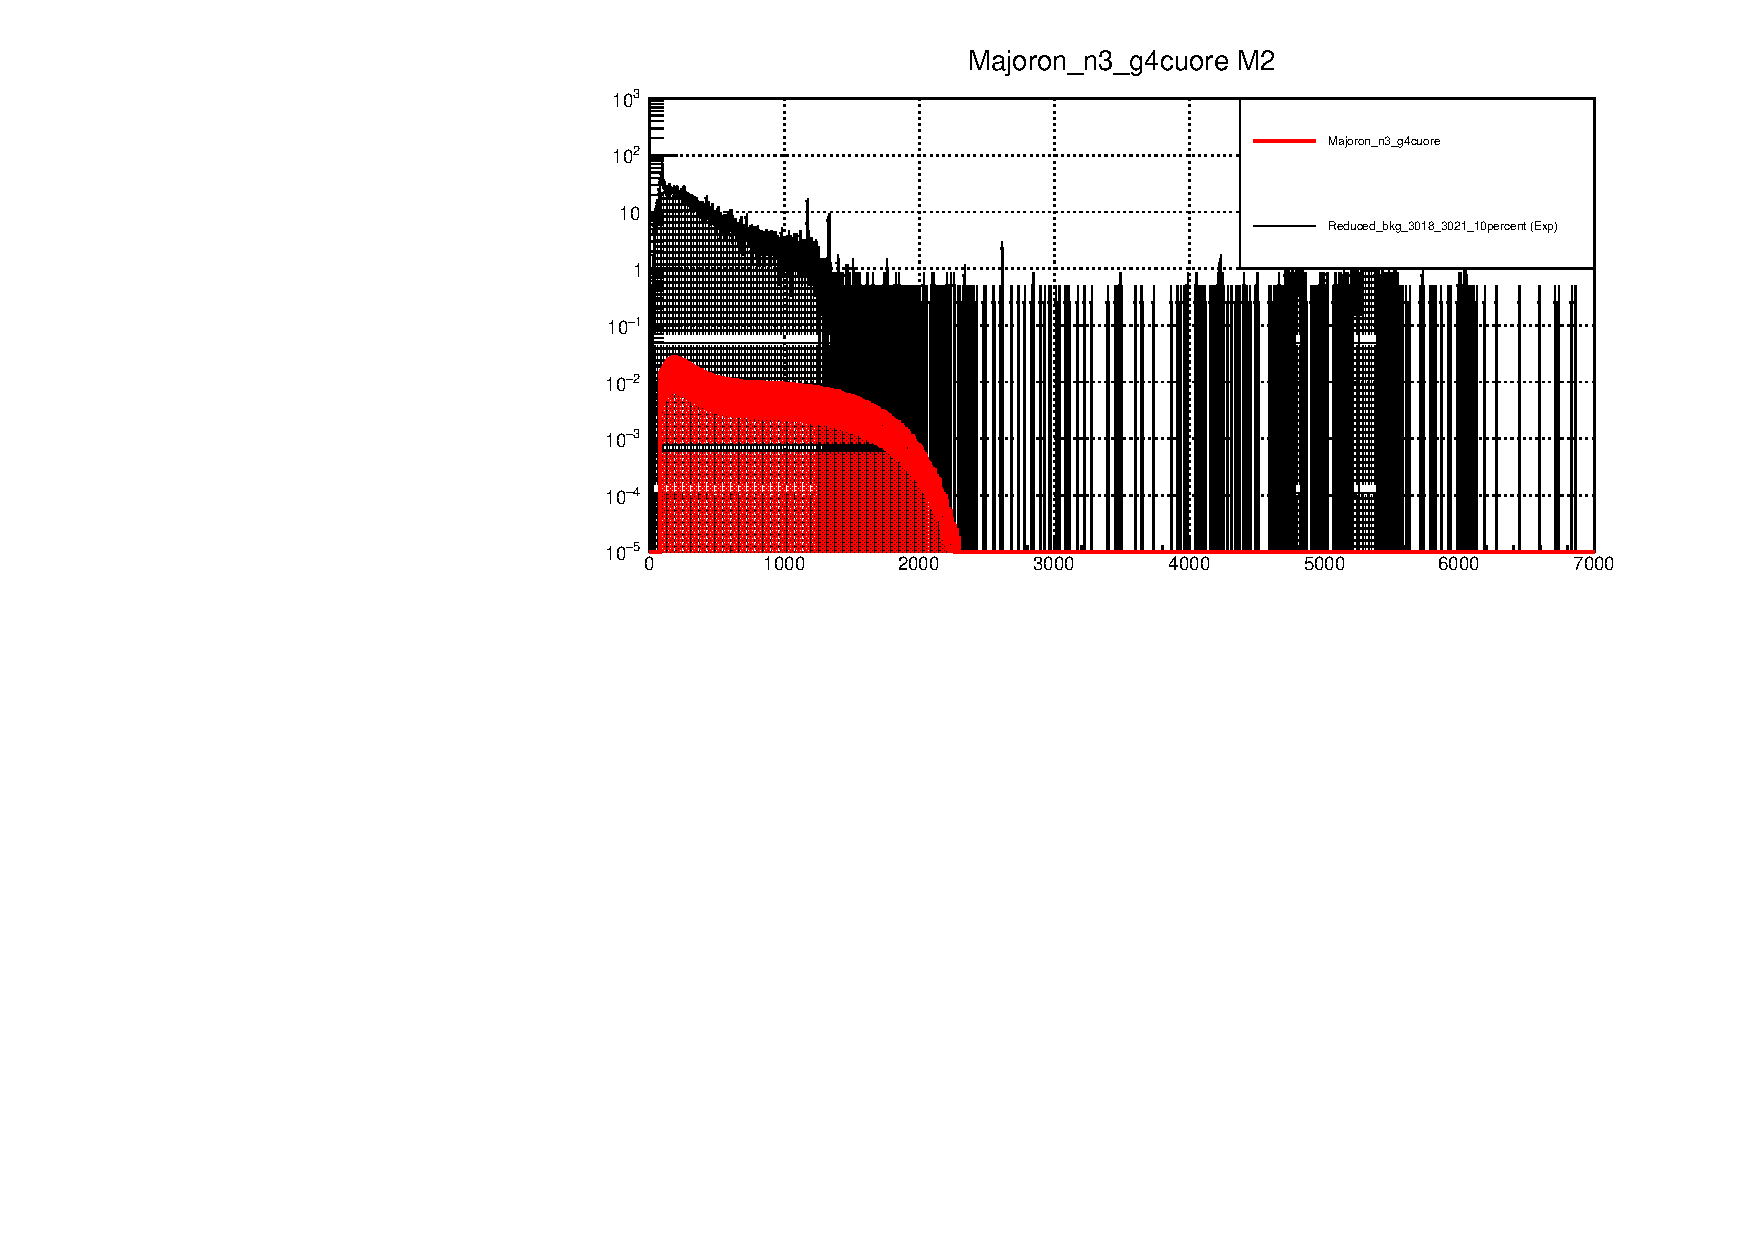
\includegraphics[width=0.9\textwidth]{Figures/Majoron_n3_g4cuore_M2.pdf}
\end{subfigure}
\qquad
\begin{subfigure}[t]{0.49\linewidth}
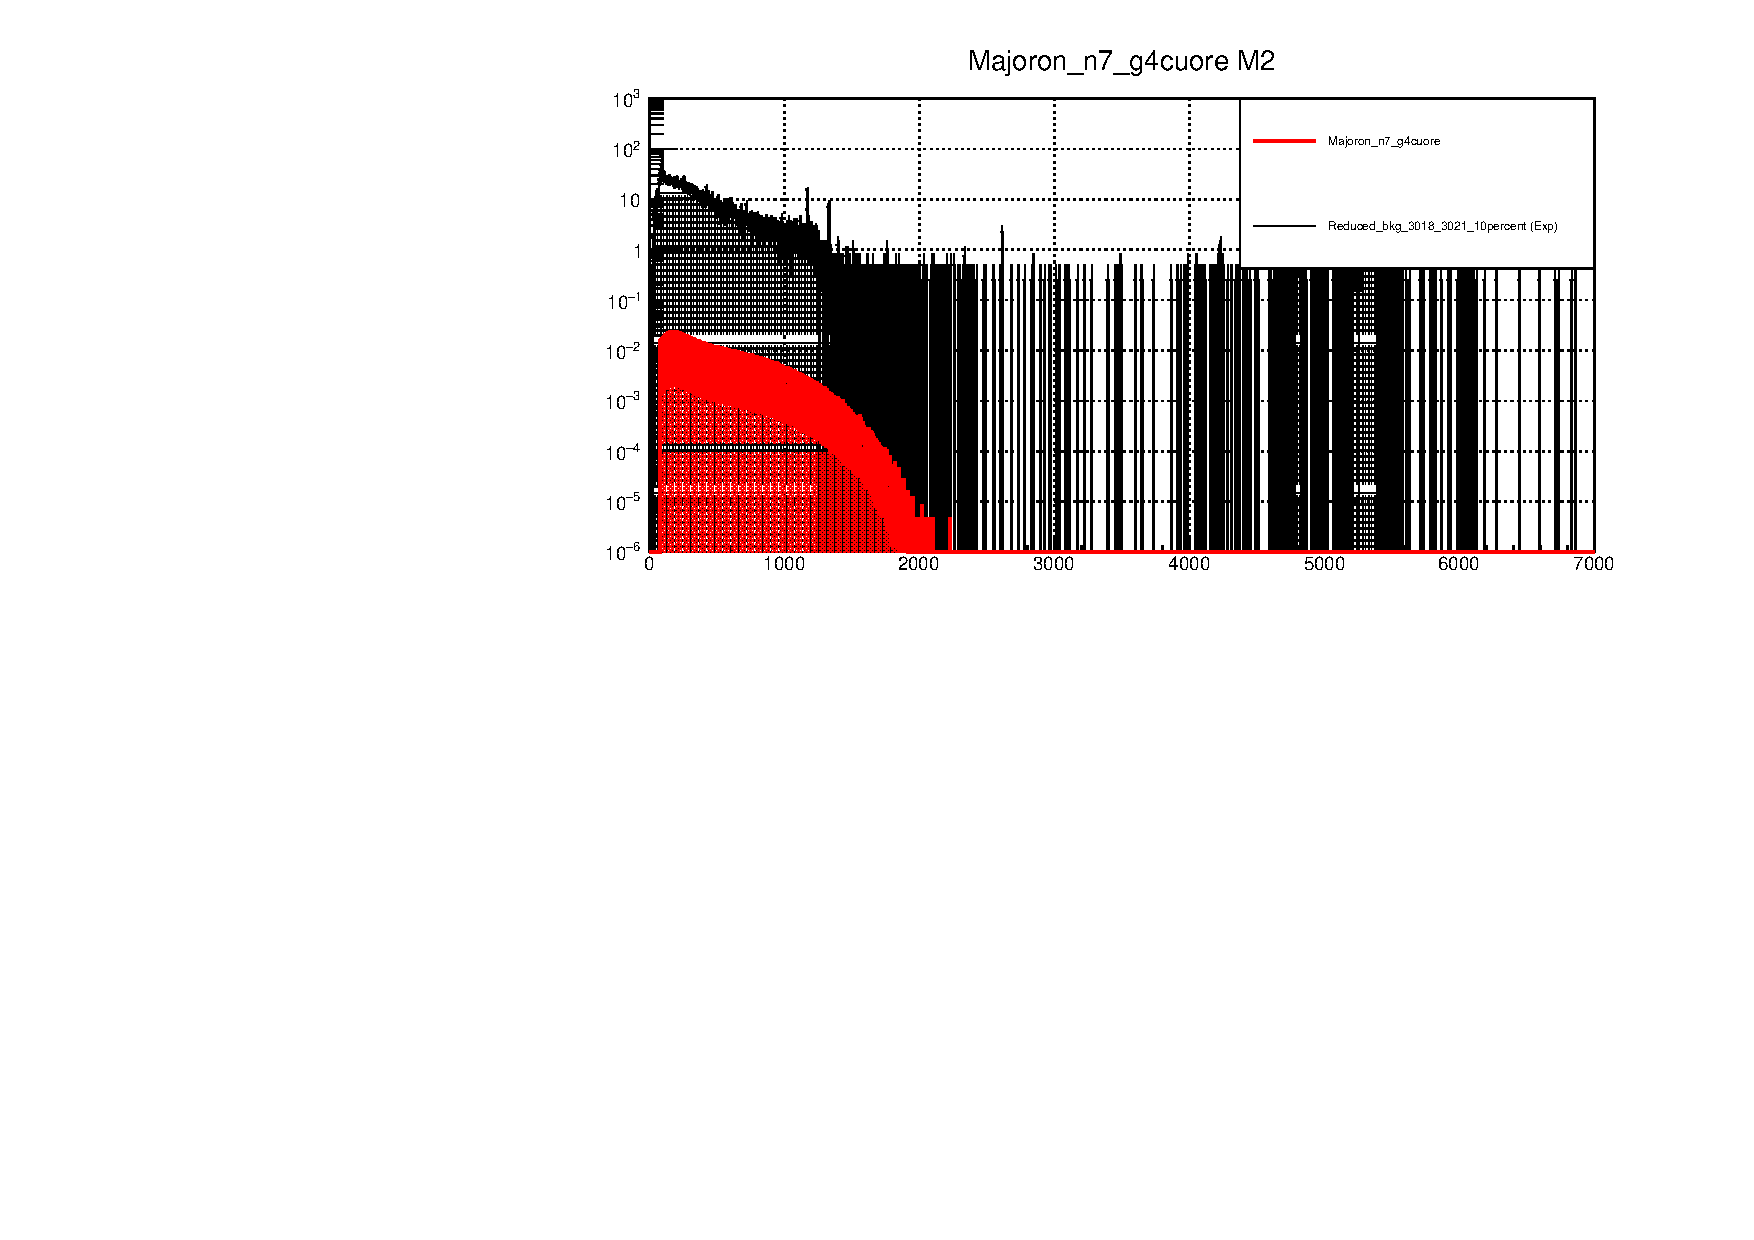
\includegraphics[width=0.9\textwidth]{Figures/Majoron_n7_g4cuore_M2.pdf}
\end{subfigure}
\caption[The fitted contribution of Majoron decays for the different spectral indices in the \Mtwo~ spectrum.]{The fitted contribution of Majoron decays for the different spectral indices in the \Mtwo~ spectrum.}
\label{fig:SpectralIndicesM2Fit}
\end{figure}

Figures to include: Correlation matrix, Fit value distributions for all the Majoron spectra, background model with only 2nu -- describe deficiencies i.e. alpha region low-E and 2 MeV, systematics (floors, layers, etc.), 